%% Преамбула TeX-файла

% 1. Стиль и язык
\documentclass[utf8x]{G7-32} % Стиль (по умолчанию будет 14pt)
\usepackage[T2A]{fontenc}
\usepackage[russian]{babel}
% Остальные стандартные настройки убраны в preamble.inc.tex.
\sloppy

% Настройки стиля ГОСТ 7-32
% Для начала определяем, хотим мы или нет, чтобы рисунки и таблицы нумеровались в пределах раздела, или нам нужна сквозная нумерация.
\EqInChapter % формулы будут нумероваться в пределах раздела
\TableInChapter % таблицы будут нумероваться в пределах раздела
\PicInChapter % рисунки будут нумероваться в пределах раздела

% Добавляем гипертекстовое оглавление в PDF
\usepackage[
bookmarks=true, colorlinks=true, unicode=true,
urlcolor=black,linkcolor=black, anchorcolor=black,
citecolor=black, menucolor=black, filecolor=black,
]{hyperref}

% Изменение начертания шрифта --- после чего выглядит таймсоподобно.
% apt-get install scalable-cyrfonts-tex

\IfFileExists{cyrtimes.sty}
    {
        \usepackage{cyrtimespatched}
    }
    {
        % А если Times нету, то будет CM...
    }

\usepackage{graphicx}   % Пакет для включения рисунков

% С такими оно полями оно работает по-умолчанию:
% \RequirePackage[left=20mm,right=10mm,top=20mm,bottom=20mm,headsep=0pt]{geometry}
% Если вас тошнит от поля в 10мм --- увеличивайте до 20-ти, ну и про переплёт не забывайте:
\geometry{right=20mm}
\geometry{left=30mm}


% Пакет Tikz
\usepackage{tikz}
\usetikzlibrary{arrows,positioning,shadows}

% Произвольная нумерация списков.
\usepackage{enumerate}

% ячейки в несколько строчек
\usepackage{multirow}

% itemize внутри tabular
\usepackage{paralist,array}


% Настройки листингов.
% 8 Листинги

\usepackage{listings}

% Значения по умолчанию
\lstset{
  basicstyle= \footnotesize,
  breakatwhitespace=true,% разрыв строк только на whitespacce
  breaklines=true,       % переносить длинные строки
%   captionpos=b,          % подписи снизу -- вроде не надо
  inputencoding=koi8-r,
  numbers=left,          % нумерация слева
  numberstyle=\footnotesize,
  showspaces=false,      % показывать пробелы подчеркиваниями -- идиотизм 70-х годов
  showstringspaces=false,
  showtabs=false,        % и табы тоже
  stepnumber=1,
  tabsize=4,              % кому нужны табы по 8 символов?
  frame=single
}

% Стиль для псевдокода: строчки обычно короткие, поэтому размер шрифта побольше
\lstdefinestyle{pseudocode}{
  basicstyle=\small,
  keywordstyle=\color{black}\bfseries\underbar,
  language=Pseudocode,
  numberstyle=\footnotesize,
  commentstyle=\footnotesize\it
}

% Стиль для обычного кода: маленький шрифт
\lstdefinestyle{realcode}{
  basicstyle=\scriptsize,
  numberstyle=\footnotesize
}

% Стиль для коротких кусков обычного кода: средний шрифт
\lstdefinestyle{simplecode}{
  basicstyle=\footnotesize,
  numberstyle=\footnotesize
}

% Стиль для BNF
\lstdefinestyle{grammar}{
  basicstyle=\footnotesize,
  numberstyle=\footnotesize,
  stringstyle=\bfseries\ttfamily,
  language=BNF
}

% Определим свой язык для написания псевдокодов на основе Python
\lstdefinelanguage[]{Pseudocode}[]{Python}{
  morekeywords={each,empty,wait,do},% ключевые слова добавлять сюда
  morecomment=[s]{\{}{\}},% комменты {а-ля Pascal} смотрятся нагляднее
  literate=% а сюда добавлять операторы, которые хотите отображать как мат. символы
    {->}{\ensuremath{$\rightarrow$}~}2%
    {<-}{\ensuremath{$\leftarrow$}~}2%
    {:=}{\ensuremath{$\leftarrow$}~}2%
    {<--}{\ensuremath{$\Longleftarrow$}~}2%
}[keywords,comments]

% Свой язык для задания грамматик в BNF
\lstdefinelanguage[]{BNF}[]{}{
  morekeywords={},
  morecomment=[s]{@}{@},
  morestring=[b]",%
  literate=%
    {->}{\ensuremath{$\rightarrow$}~}2%
    {*}{\ensuremath{$^*$}~}2%
    {+}{\ensuremath{$^+$}~}2%
    {|}{\ensuremath{$|$}~}2%
}[keywords,comments,strings]

% Подписи к листингам на русском языке.
\renewcommand\lstlistingname{\cyr\CYRL\cyri\cyrs\cyrt\cyri\cyrn\cyrg}
\renewcommand\lstlistlistingname{\cyr\CYRL\cyri\cyrs\cyrt\cyri\cyrn\cyrg\cyri}


% Полезные макросы листингов.
% Любимые команды
\newcommand{\Code}[1]{\textbf{#1}}


\title{Разработка технологии управления распределенной системой “умного освещения” с элементами искусственного интеллекта}
\author{Егор Соловьев }
\date{02.03.2015}

\begin{document}


% Команды \breakingbeforechapters и \nonbreakingbeforechapters
% управляют разрывом страницы перед главами.
% По-умолчанию страница разрывается.

% \nobreakingbeforechapters
% \breakingbeforechapters


 

\chapter{Защита интеллектуальной собственности}
 \section{Формула изобретения}
 
1. Способ управления освещением заключающийся в том, что 

ставят в соответствие команды, передаваемые через локальную или глобальную сеть на устройство освещения управляющим командам, формируемым на устройстве управления освещением, 

формируют команды управления освещением,

определяют номера устройств и команды управления освещением

в соответствии с полученной командой управления формируют световую картинку одним или несколькими осветительными устройствами 

\textbf{отличающийся тем, что для формирования команд управления освещением }

выполняют жест устройством, содержащим компоненты регистрации ускорений,

регистрируют проекцию ускорения на некоторые выбранные оси в некоторых точках устройства - манипулятора как функцию времени,

преобразуют проекцию ускорения в массив данных, 

передают массив данных на облачный сервер,

вычисляют код жеста, поставленный в соответствие переданного массива данных,

определяют набор команд, которые должны быть активизированы по результатам определения жеста,

передают команды на осветительное устройство, 


 
 
2. Система управления освещением, реализующая способ управления освещением, включающая в себя:


устройство, имеющее название, включающее корпус, вычислительный модуль, модуль передачи данных по беспроводному каналу, модуль передачи данных (имеющий доступ в интернет),   

сервер, подключенный к сети интернет,

устройство, включающее корпус, вычислительный модуль, модуль передачи данных по беспроводному каналу, модуль передачи данных  (имеющий доступ в интернет),  

одно или несколько осветительных устройств, каждое из которых включает, вычислительный модуль, модуль передачи данных, один или несколько осветителей (ламп),


мобильный телефон с установленным на нем специальным мобильным приложением,

\textbf{при этом}



\textbf{отличающееся тем, что в состав системы управления освещением дополнительно включено}

устройство "волшебная палочка", включающее  вычислительный модуль,  один или несколько акселерометров и модуль передачи данных по беспроводному каналу, корпус,

\textbf{при этом }
модуль передачи данных по беспроводному каналу устройства "волшебная палочка" соединен по безвоздушной линии передачи данных с модулем передачи данных по беспроводному каналу устройства, включающее корпус, вычислительный модуль, модуль передачи данных по беспроводному каналу, модуль передачи данных  (имеющий доступ в интернет),

2. Система по пункту 1, отличающаяся тем, что два устройства, включающие корпус, вычислительный модуль, модуль передачи данных по беспроводному каналу, модуль передачи данных (имеющий доступ в интернет) объединены в один.


\section{Описание изобретения}

Изобретение "Способ управления освещением и система для его реализации" относится к коду H05B 37/02 МПК 

 
\subsection{Область техники, к которой относится изобретение}

Изобретение относится к области бытовых электрических приборов, в частности - к бытовым осветительным приборам.



\subsection{Раскрытие сущности изобретения}
1. Предложен способ управления освещением, заключающийся в том, что для управления "умным осветителем" разрабатывают набор команд управления состоянием осветительного устройства. 

В качестве такого устройства может использоваться, например "умная лампа" компании XIAOMI 

Она управляется командами через REST протокол.

При получении такой команды лампа светится синим цветом, соответствующим RGB тройке



ставят в соответствие команды, передаваемые через локальную или глобальную сеть на устройство освещения управляющим командам, формируемым на устройстве управления освещением, 

формируют команды управления освещением,

определяют номера устройств и команды управления освещением

в соответствии с полученной командой управления формируют световую картинку одним или несколькими осветительными устройствами 

\textbf{отличающийся тем, что для формирования команд управления освещением }

выполняют жест устройством, содержащим компоненты регистрации ускорений,

регистрируют проекцию ускорения на некоторые выбранные оси в некоторых точках устройства - манипулятора как функцию времени

преобразуют проекцию ускорения в массив данных, 

передают массив данных на облачный сервер

вычисляют код жеста, поставленный в соответствие переданного массива данных,

определяют набор команд, которые должны быть активизированы по результатам определения жеста,

передают команды на осветительное устройство, 



2. Предложена система управления освещением, включающая   
устройство 2, включающее корпус , вычислительный модуль, модуль передачи данных по беспроводному каналу, модуль передачи данных  (имеющий доступ в интернет),   

сервер 3, подключенный к сети интернет,

устройство 4, включающее корпус , вычислительный модуль, модуль передачи данных по беспроводному каналу, модуль передачи данных  (имеющий доступ в интернет),  

одно или несколько осветительных устройств 5,   каждое из которых включает, вычислительный модуль, модуль передачи данных, один или несколько осветителей (ламп),


мобильный телефон 6 с установленным на нем специальным мобильным приложением,

\textbf{при этом}



\textbf{отличающееся тем, что в состав системы управления освещением дополнительно включено}

устройство "волшебная палочка"  1, включающее  вычислительный модуль 1.1,  один или несколько акселерометров 1.2 и модуль передачи данных по беспроводному каналу 1.3, корпус,

\textbf{при этом }
модуль передачи данных по беспроводному каналу 1.3 устройства "волшебная палочка" соединен по безвоздушной линии передачи данных с модулем передачи данных по беспроводному каналу 2.2 устройства 2,

В качестве вычислительного модуля может быть использован вычислительный модуль на основе процессора 

В качестве акселерометра 1.2 может быть, например, использован акселерометрический блок 9250 компании Texas Instruments. 
 

\subsection{Краткое описание чертежей (если они содержатся в заявке)}
1. Система по пункту 1
На фиг.1 приведена блок схема описывающая способ управления освещением.

\begin{figure}[ht]
   \centering
   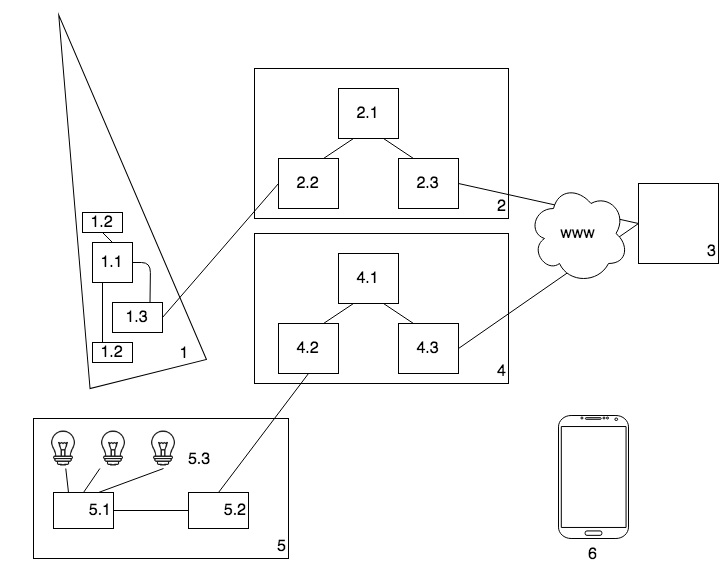
\includegraphics[scale=.4]{figures/patent-Magget-egor}
    \caption{Принципиальная схема системы 1}
    \label{patent-Magget-egor}
\end{figure}


Система включает 

устройство 2, включающее корпус , вычислительный модуль, модуль передачи данных по беспроводному каналу, модуль передачи данных  (имеющий доступ в интернет),   

сервер 3, подключенный к сети интернет,

устройство 4, включающее корпус , вычислительный модуль, модуль передачи данных по беспроводному каналу, модуль передачи данных  (имеющий доступ в интернет),  

одно или несколько осветительных устройств 5,   каждое из которых включает, вычислительный модуль, модуль передачи данных, один или несколько осветителей (ламп),


мобильный телефон 6 с установленным на нем специальным мобильным приложением,

\textbf{при этом}



\textbf{отличающееся тем, что в состав системы управления освещением дополнительно включено}

устройство "волшебная палочка"  1, включающее  вычислительный модуль 1.1,  один или несколько акселерометров 1.2 и модуль передачи данных по беспроводному каналу 1.3, корпус,

\textbf{при этом }
модуль передачи данных по беспроводному каналу 1.3 устройства "волшебная палочка" соединен по безвоздушной линии передачи данных с модулем передачи данных по беспроводному каналу 2.2 устройства 2,

На фиг.2  приведен пример сигнала на выходе акселерометра.

\begin{figure}[ht]
   \centering
   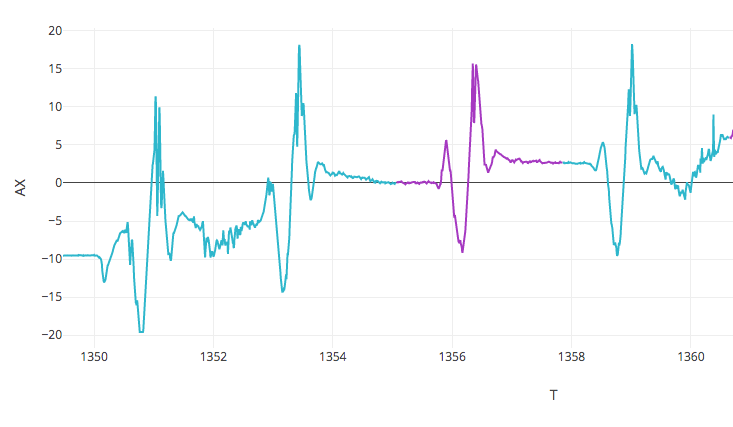
\includegraphics[scale=.5]{figures/AX-demo.png}
    \caption{Сигнал на выходе акселерометра}
    \label{fig:AX-data}
\end{figure}

%\begin{figure}[h]
 %  \centering
%   \includegraphics[scale=.4]{figures/fig2-accelerometer_data}
 %%%\end{figure}

2. Система по пункту 1, отличающаяся тем, что устройство 2 и устройство 4 совмещены.

\subsection{Осуществление изобретения}  

1. Способ управления освещением реализуется следующим образом.

Выполняют жест устройством 1, содержащим компоненты регистрации ускорений 1.2, регистрируют проекцию ускорения на некоторые выбранные оси в некоторых точках устройства - манипулятора как функцию времени. С помощью вычислительного модуля 1.1 преобразуют проекцию ускорения в массив данных. С помощью модуля передачи данных по беспроводному каналу 1.3 передают массив данных на облачный модуль передачи данных по беспроводному каналу 2.2 устройства 2. Массив данных, пройдя через вычислительный модуль 2.1, а затем через модуль передачи данных по беспроводному каналу 2.3 (имеющий доступ в интернет), передают на облачный сервер 3. Сервер снабжают нейронной сетью, способной вычислять код жеста, поставленный в соответствие переданного массива данных. Также на сервере определяют набор команд, которые должны быть активизированы по результатам определения жеста. Передается набор команд на осветительное устройство посредством устройства 4, аналогичным по своему составу устройству 2. Передают на осветительное устройство команды через модуль передачи данных 5.2. Затем данные через вычислительный модуль 5.1 распределяют по соответствующим данным лампочкам 5.3. Через лампочки  воспроизводят световой сигнал.

2. Система работает следующим образом.

При выполнении жеста, устройство 1, содержащее компоненты регистрации ускорений 1.2, регистрирует проекцию ускорения на некоторые выбранные оси в некоторых точках устройства - манипулятора как функцию времени. Вычислительный модуля 1.1 преобразуют проекцию ускорения в массив данных. Модуль передачи данных по беспроводному каналу 1.3 передает массив данных на облачный модуль передачи данных по беспроводному каналу 2.2 устройства 2. Массив данных, пройдя через вычислительный модуль 2.1, а затем через модуль передачи данных по беспроводному каналу 2.3 (имеющий доступ в интернет), приходит на облачный сервер 3. 

Сервер снабжен нейронной сетью, способной вычислять код жеста, поставленный в соответствие переданного массива данных. Также на сервере определяют набор команд, которые должны быть активизированы по результатам определения жеста. Устройство 4 передает набор команд на осветительное устройство посредством, аналогичным по своему составу устройству 2. Осветительное устройство, получает команды через модуль модуль передачи данных 5.2. Затем данные через вычислительный модуль 5.1 распределяются по соответствующим данным лампочкам 5.3. Лампочки воспроизводят световой сигнал.
 

 
 
% % Список литературы при помощи BibTeX
% Юзать так:
%
% pdflatex rpz
% bibtex rpz
% pdflatex rpz

\bibliographystyle{gost780u}
\bibliography{smartlight}

%%% Local Variables: 
%%% mode: latex
%%% TeX-master: "rpz"
%%% End: 
      % Список литературы 

 

\end{document}

%%% Local Variables:
%%% mode: latex